\documentclass[twoside, 12pt]{article}
\usepackage{amsmath}
\usepackage{lipsum} % Package to generate dummy text throughout this template
\usepackage[english]{isodate}% http://ctan.org/pkg/isodate
\usepackage{pgfgantt}
\usepackage[show]{ed}
\setlength{\parindent}{0pt}
\usepackage[sc]{mathpazo} % Use the Palatino font
\usepackage[T1]{fontenc} % Use 8-bit encoding that has 256 glyphs
\linespread{1.2} % Line spacing - Palatino needs more space between lines
\usepackage{microtype} % Slightly tweak font spacing for aesthetics
\usepackage{minted}
\usepackage{enumitem}
\usepackage{listings}
\usepackage[section]{placeins}
\usepackage{nameref}
\usemintedstyle{autumn}
\usepackage[hmarginratio=1:1,top=32mm,left=25mm,right=25mm,columnsep=18pt,bottom=27mm]{geometry} % Document margins
\usepackage{multicol} % Used for the two-column layout of the document
\usepackage[hang, small,labelfont=bf,up,textfont=it,up]{caption} % Custom captions under/above floats in tables or figures
\usepackage{booktabs} % Horizontal rules in tables
\usepackage{float} % Required for tables and figures in the multi-column environment - they need to be placed in specific locations with the [H] (e.g. \begin{table}[H])
\usepackage{hyperref} % For hyperlinks in the PDF
\usepackage{xspace}
\usepackage{lettrine} % The lettrine is the first enlarged letter at the beginning of the text
\usepackage{paralist} % Used for the compactitem environment which makes bullet points with less space between them
\usepackage{etoolbox}
\usepackage{eurosym}
\patchcmd{\thebibliography}{\section*{\refname}}{}{}{}
\usepackage{abstract} % Allows abstract customization
\renewcommand{\abstractnamefont}{\normalfont\bfseries} % Set the "Abstract" text to bold
\renewcommand{\abstracttextfont}{\normalfont\small\itshape} % Set the abstract itself to small italic text

\usepackage{titlesec} % Allows customization of titles
%\renewcommand\thesection{\Roman{section}} % Roman numerals for the sections
%\renewcommand\thesubsection{\Roman{subsection}} % Roman numerals for subsections
\titleformat{\section}[block]{\large\scshape\centering\bfseries}{\thesection.}{1em}{} % Change the look of the section titles
\titleformat{\subsection}[block]{\large\scshape}{\thesubsection.}{1em}{} % Change the look of the section titles
\usepackage{cite}
\usepackage{fancyhdr} % Headers and footers
\pagestyle{fancy} % All pages have headers and footers
\fancyhead{} % Blank out the default header
\fancyfoot{} % Blank out the default footer
\fancyhead[C]{Naomi Pentrel $\cdot$ \href{mailto:n.pentrel@jacobs-university.de}{n.pentrel@jacobs-university.de} $\cdot$ \today} % Custom header text
\fancyfoot[RO,LE]{\thepage} % Custom footer text
\usepackage{graphicx}
\usepackage{wrapfig}
\usepackage[]{natbib}
\usepackage{tocloft}
\renewcommand*{\figureautorefname}{figure}
\def\stex{\texorpdfstring{\raisebox{-.5ex}S\kern-.5ex\TeX}{sTeX}\xspace}
\def\sTeX{\stex}

\definecolor{mygreen}{rgb}{0,0.6,0}
\definecolor{mygray}{rgb}{0.5,0.5,0.5}
\definecolor{mymauve}{rgb}{0.58,0,0.82}


\lstset{ %
  backgroundcolor=\color{white},   % choose the background color; you must add \usepackage{color} or \usepackage{xcolor}
  basicstyle=\footnotesize,        % the size of the fonts that are used for the code
  breakatwhitespace=false,         % sets if automatic breaks should only happen at whitespace
  breaklines=true,                 % sets automatic line breaking
  captionpos=b,                    % sets the caption-position to bottom
  commentstyle=\color{mygreen},    % comment style
  deletekeywords={...},            % if you want to delete keywords from the given language
  escapeinside={\%*}{*)},          % if you want to add LaTeX within your code
  extendedchars=true,              % lets you use non-ASCII characters; for 8-bits encodings only, does not work with UTF-8
  frame=single,                    % adds a frame around the code
  keepspaces=true,                 % keeps spaces in text, useful for keeping indentation of code (possibly needs columns=flexible)
  keywordstyle=\color{blue},       % keyword style
  language=Octave,                 % the language of the code
  otherkeywords={*,...},            % if you want to add more keywords to the set
  numbers=left,                    % where to put the line-numbers; possible values are (none, left, right)
  numbersep=5pt,                   % how far the line-numbers are from the code
  numberstyle=\tiny\color{mygray}, % the style that is used for the line-numbers
  rulecolor=\color{black},         % if not set, the frame-color may be changed on line-breaks within not-black text (e.g. comments (green here))
  showspaces=false,                % show spaces everywhere adding particular underscores; it overrides 'showstringspaces'
  showstringspaces=false,          % underline spaces within strings only
  showtabs=false,                  % show tabs within strings adding particular underscores
  stepnumber=2,                    % the step between two line-numbers. If it's 1, each line will be numbered
  stringstyle=\color{mymauve},     % string literal style
  tabsize=2,                       % sets default tabsize to 2 spaces
  title=\lstname                   % show the filename of files included with \lstinputlisting; also try caption instead of title
}


\usepackage{quoting}
\quotingsetup{vskip=50pt}

%\usepackage{csquotes}
%\MakeOuterQuote{"}

\hypersetup{
    bookmarks=true,
    unicode=false,
    pdftoolbar=true,
    pdfmenubar=true,
    pdffitwindow=false,
    pdfstartview={FitH},
    pdftitle={My title},
    pdfauthor={Author},
    pdfsubject={Subject},
    pdfcreator={Creator},
    pdfproducer={Producer},
    pdfkeywords={keyword1} {key2} {key3},
    pdfnewwindow=true,
    colorlinks=false,
    %linkcolor=red,
    %citecolor=green,
    %filecolor=magenta,
    %urlcolor=cyan
    pdfborder={0 0 0},
}


\usepackage{caption}
\usepackage{subcaption}
\usepackage[section]{placeins}
\usepackage{qtree}
\usepackage{gensymb}

\usepackage{setspace}

\usepackage{color}

%\doublespacing
% or:
%\onehalfspacing

%\renewcommand\cftchapafterpnum{\vskip10pt}
%\renewcommand\cftsecafterpnum{\vskip15pt}

%----------------------------------------------------------------------------------------
%	TITLE SECTION
%----------------------------------------------------------------------------------------

\title{\vspace{-15mm}\fontsize{24pt}{10pt}\selectfont\textbf{// All comments are NOT created equal}} % Article title


\newenvironment{myfont}{\fontfamily{\sfdefault}\selectfont}{\par}

%----------------------------------------------------------------------------------------
% Macros
%----------------------------------------------------------------------------------------
\newcommand{\sys}{\textsc{RPresentation}\xspace}

%----------------------------------------------------------------------------------------

\begin{document}
\thispagestyle{empty}
\pagenumbering{roman}
\begin{flushright}
    
\includegraphics[scale=1.0]{assets/Logo}
  \end{flushright}
  \vspace{20mm}
  \begin{center}
    \huge
    \textbf{Autonomous Coastline Exploration with a Focus on Reef Structures}
  \end{center}
  \vspace*{4mm}
  \begin{center}
   \Large by
  \end{center}
  \vspace*{4mm}
  \begin{center}
    \Large
    \textbf{Naomi Pentrel \& Denis Rochau}
  \end{center}
  \vspace*{20mm}
  \begin{center}
    \large
    Advanced Robotics
  \end{center}
  \vfill
  \begin{flushright}
    \large
    \begin{tabular}{l}
      
      \hline
      Prof. Dr. Andreas Birk\\
      \\
    \end{tabular}
  \end{flushright}
  \vspace*{8mm}
  \begin{flushleft}
    \large
    Date of Submission: \today \\
    \rule{\textwidth}{1pt}
  \end{flushleft}
  \begin{center}
    \Large Jacobs University Bremen - School of Engineering and Science
  \end{center}

\newpage

\thispagestyle{fancy} % All pages have headers and footers

%----------------------------------------------------------------------------------------
%	ARTICLE CONTENTS
%----------------------------------------------------------------------------------------

 \section*{Abstract}
 \label{sec:abstract}
 
Mappings of underwater reef structures are needed in different fields. Regardless of why we want to explore underwater reefs, when exploring them we need a strategy to map them. The strategy we use for mapping the reef should accomplish two things: it should collect the data for the whole area we are interested in and it should keep our robot safe while it explores the area.\\

The strategy we will explore in this paper goes along the reef in an iterative manner as it creates the map. As such it starts at a position on the top right of the map and works its way down. When it senses the ground or has gone far enough according to our specifications, it will move horizontally to an unexplored piece of the reef and go back up. After reaching the initial height it will again move horizontally to an unexplored piece of the reef and continue our algorithm.\\

To get a good mapping of the reef and keep the robot safe at the same time we have to optimize the above algorithm. The detailed algorithm and the suggested optimizations will be explored in this paper. The result will be an algorithm that allows the sequential mapping of 3D structures underground.\\

\newpage
\tableofcontents

\clearpage

\newpage
\thispagestyle{empty}
\topskip0pt
\vspace*{\fill}
\begin{center}

\vspace*{4cm}

\centering

\begin{quoting}
\begin{center}
\noindent
\textit{At this point, we would like to thank Prof. Dr. Birk and Ravi Rathnam for helping and supporting us during this research project.\\}
\end{center}
\end{quoting}

\vspace*{\fill}
\end{center}

\newpage
\pagenumbering{arabic}

\section{Introduction}
\label{sec:introduction}

When mapping underwater reef structures we care about the completeness of the map, as well as the optimization of the path the robot takes as it scans the reef. To achieve this we will start with a very basic algorithm. As we test this algorithm on a test reef, we will eliminate errors and improve the algorithm as needed.\\

\begin{wrapfigure}{r}{0.5\textwidth}
\vspace{-26pt}
  \begin{center}
  \fbox{
    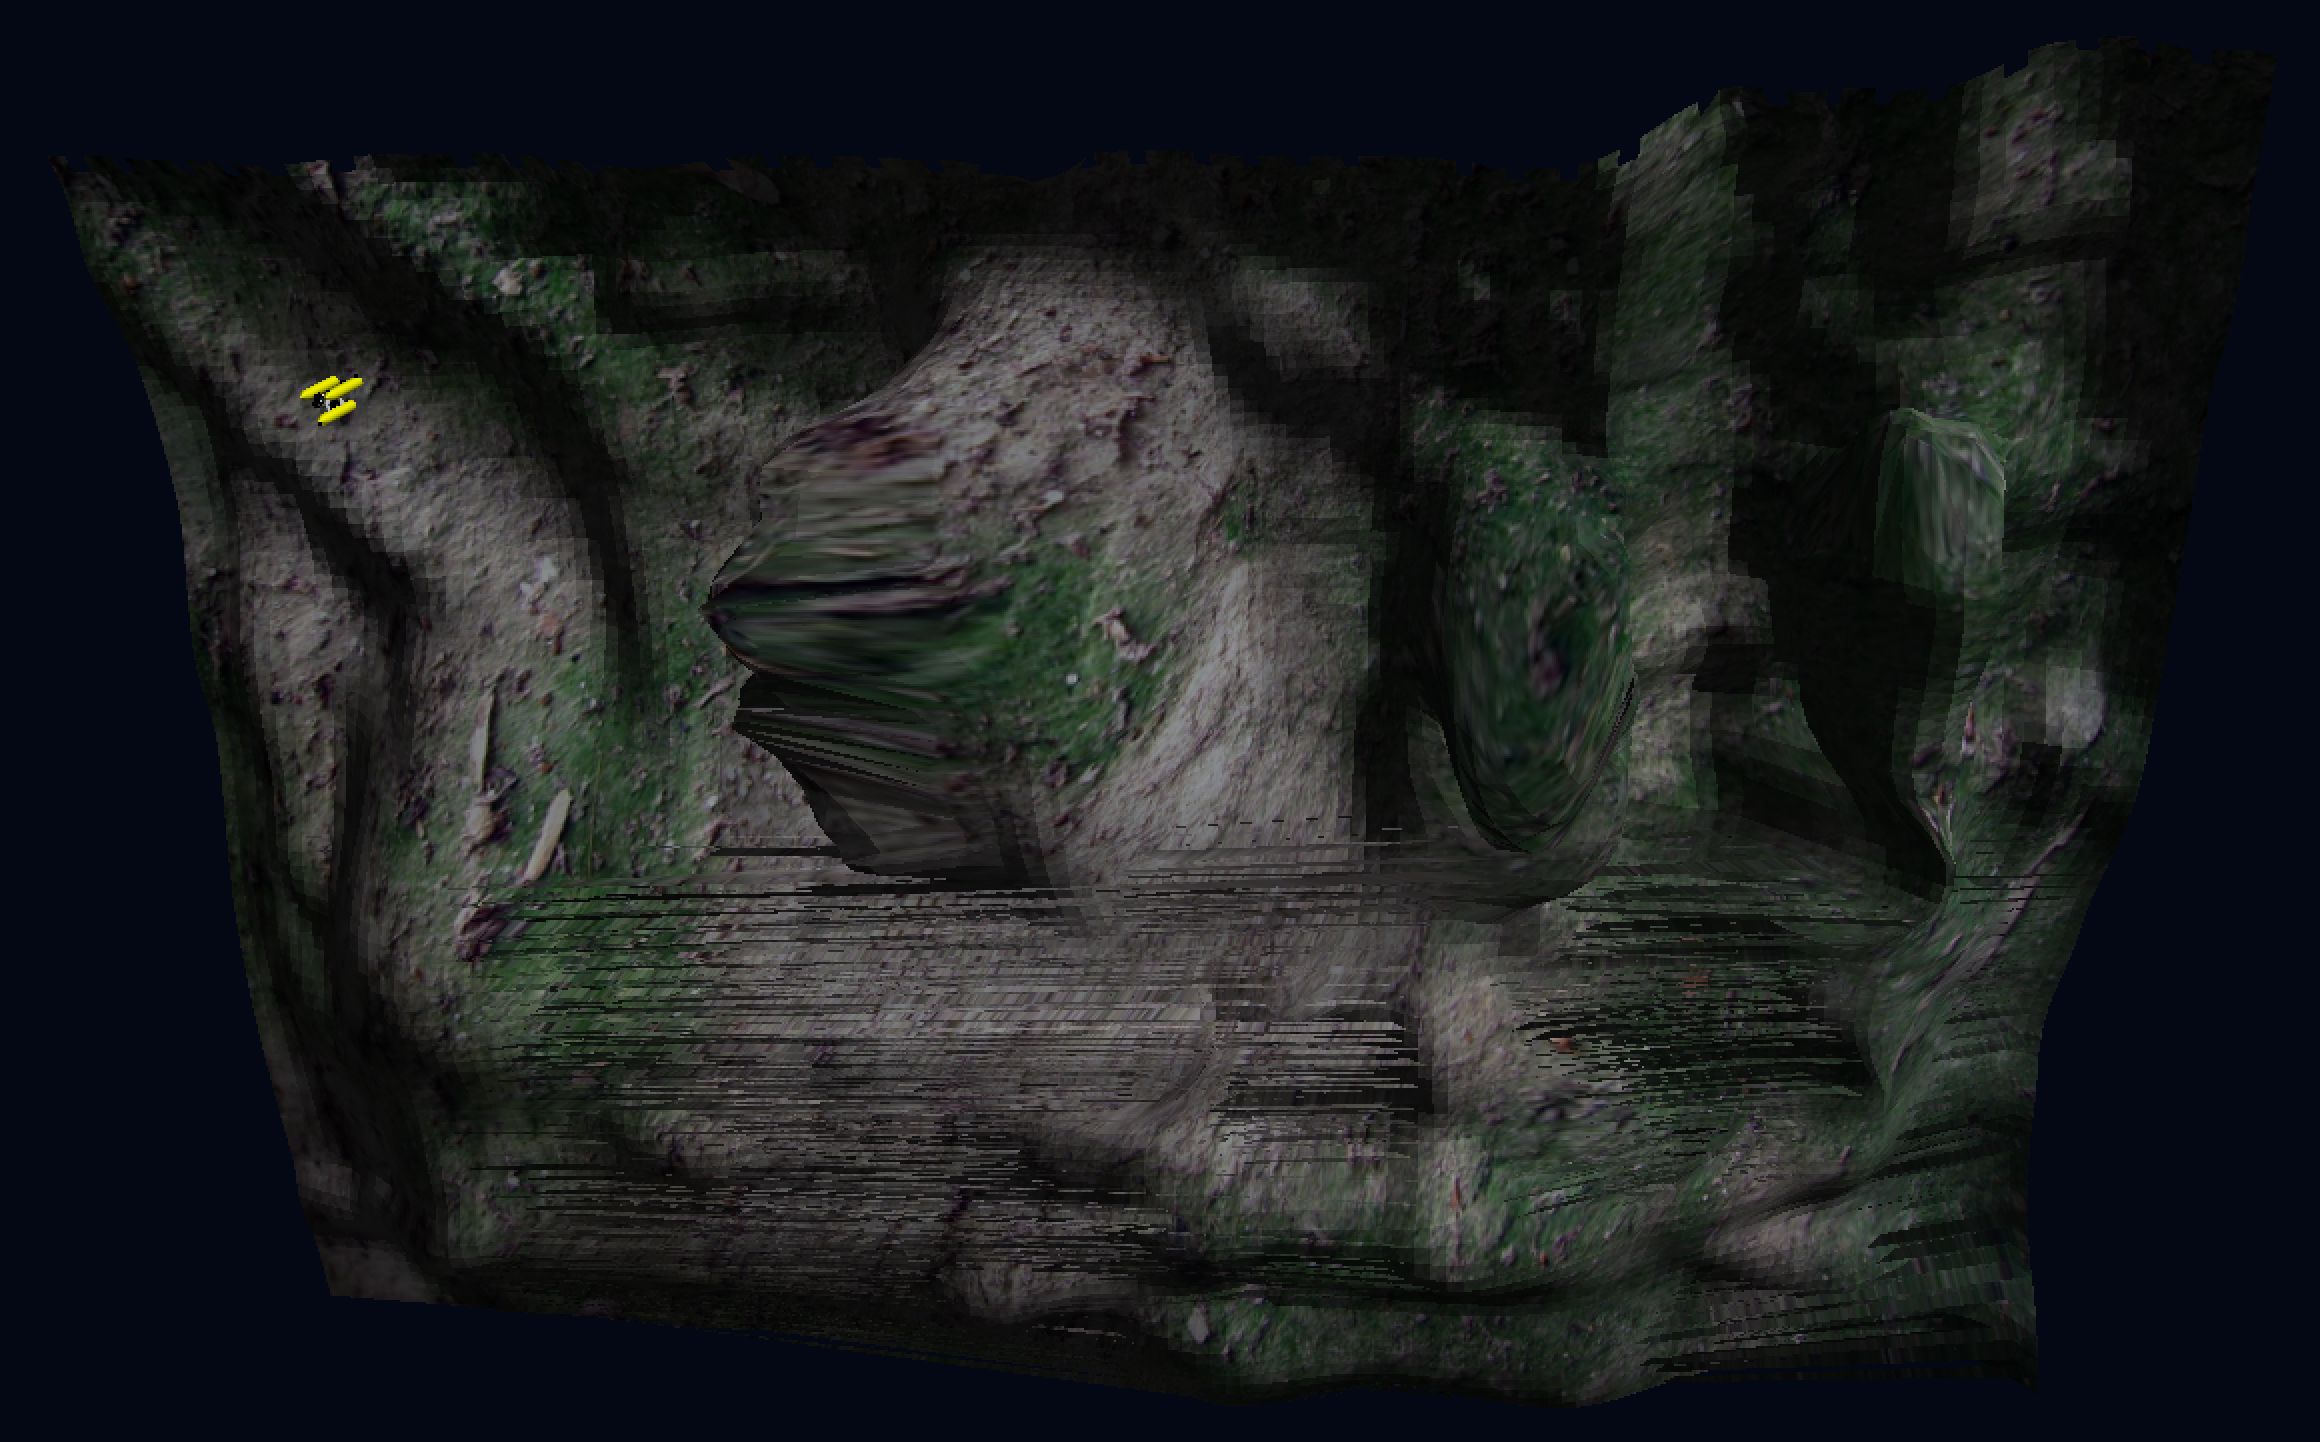
\includegraphics[width=0.48 \textwidth]{assets/reefOriginal}
    }
  \end{center}
\vspace{-20pt}
  \caption{Underwater Reef}
  \label{fig:reef}
\vspace{-10pt}
\end{wrapfigure}

We will be exploring the reef shown in \autoref{fig:reef} as a test. The idea of the basic algorithm that we will be using is shown in \autoref{fig:basicAlgorithm}. The robot starts in its starting position as shown in \autoref{fig:basicAlgorithm}. From there it will start scanning and move downwards until it either reaches the ground or a predefined \textit{maxDepth}. Once we reach that point the robot will move to the right for a predefined distance \textit{d}. At that point the robot goes back up until it reaches the predefined startDepth where it will go to the right for a predefined distance \textit{d}. This sequence is repeated until we reach the maxWidth.\\

\begin{wrapfigure}{c}{\textwidth}
\vspace{-26pt}
  \begin{center}
  \fbox{
    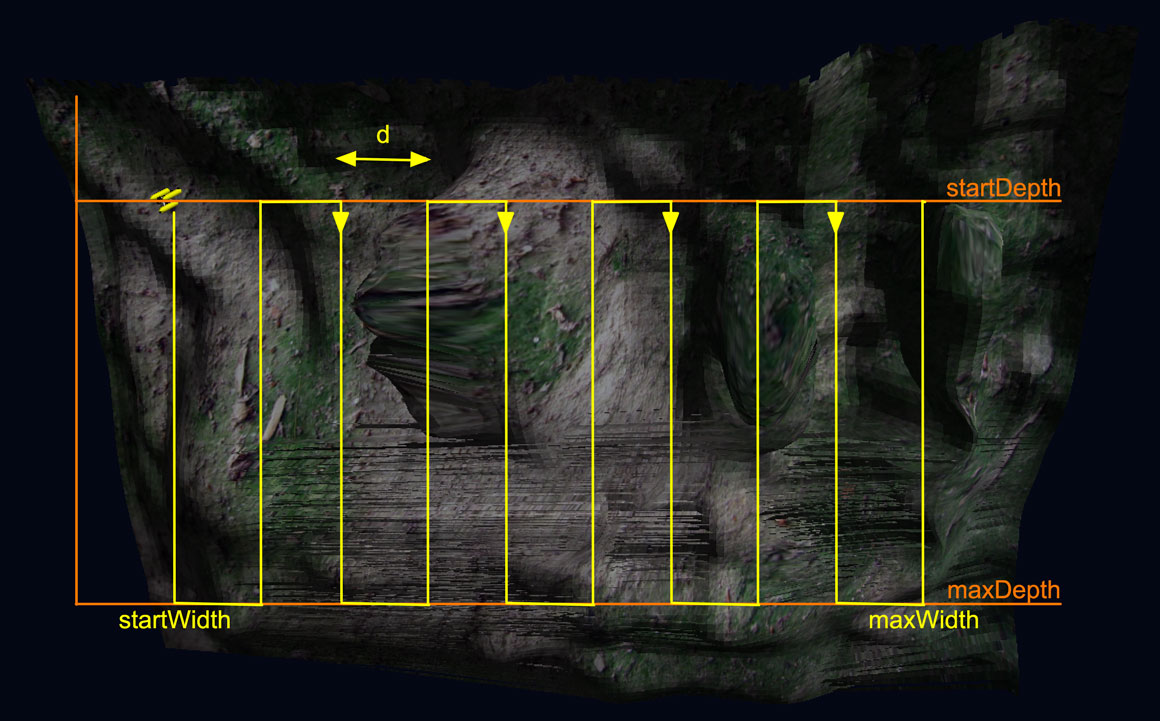
\includegraphics[width=0.90\textwidth]{assets/reefBasicAlgorithm.jpg}
    }
  \end{center}
\vspace{-20pt}
  \caption{Basic Algorithm}
  \label{fig:basicAlgorithm}
\end{wrapfigure}

\begin{wrapfigure}{l}{\textwidth}
\vspace{-50pt}
\end{wrapfigure}

Obviously the above algorithm only illustrates the basic idea. In reality, we have to also make sure the robot can actually move the way the algorithm wants it to move. Additionally, the robot should actually not be too far away from the reef so that it can scan the reef. In this paper we will therefore start from the basic algorithm discussed above and incrementally optimize until it successfully scans the reef. \\

\section{Related Work}
\label{sec:relatedworks}

\ednote{DENIS DOES THIS.}
  
\section{Preliminaries}
\label{sec:preliminaries}

\subsection{a}

\subsection{b}

\subsection{c}
\newpage
\section{Towards an Optimal Scanning Algorithm}
\label{sec:optimalScanningAlgorithm}

Looking back to the initial idea of the algorithm which we illustrated in \autoref{sec:introduction}, we will now explore how to improve on this algorithm. First we will ensure that the robot always keeps a minimum distance to the reef while also not being too far away from the reef.\\

\subsection{Distance Between Robot and Reef}

\begin{wrapfigure}{l}{0.27\textwidth}
\vspace{-28pt}
  \begin{center}
  \fbox{
    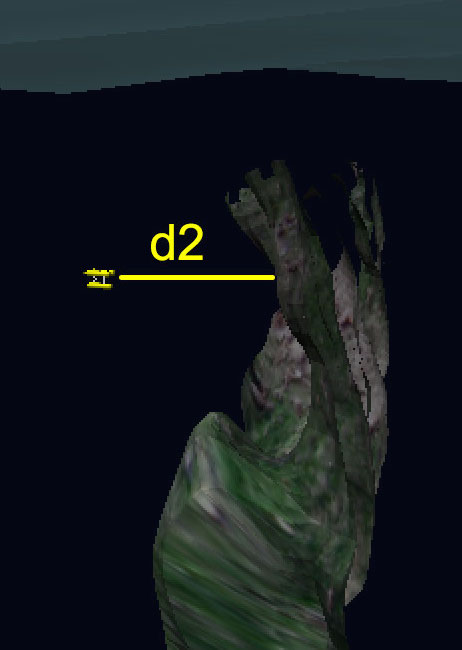
\includegraphics[width=0.25 \textwidth]{assets/reefSideways.jpg}
    }
  \end{center}
\vspace{-20pt}
  \caption{Reef Sideways}
  \label{fig:reef}
\vspace{20pt}
\end{wrapfigure}

If the robot starts in a random position, it is in our interest to get close enough to the reef to be able to scan the reef. Therefore we will move in the direction of the reef. To do this we use the following logic to check whether the robot is far enough away from the cliff to not crash but close enough to scan the cliff (see \autoref{fig:codeDistance}). Ideally the robot should always stay at exactly the \textit{minimumDistanceValue $\pm$ offset}. The \textit{scanDistance} is the scanned point of the reef that is closest to the robot.\\

\begin{wrapfigure}{c}{\textwidth}
\vspace{12pt}
\begin{lstlisting}[language=C++]
void ExploreAlgorithm::controlDistanceToCliff() {
    if(minimumDistanceValue > scanDistance) {
        moveTowardsCliff(); 
    } else if(minimumDistanceValue < (scanDistance - offset)) {
    	   moveAwayFromCliff();
    } 
}
\end{lstlisting} 
\vspace{-38pt}
  \caption{Pseudocode Snippet to Show how to Control the Distance to the Cliff}
  \label{fig:codeDistance}
  \vspace{20pt}
\end{wrapfigure}

\begin{wrapfigure}{l}{\textwidth}
\vspace{-50pt}
\end{wrapfigure}

The robot does not start to descend until it is within the specified distance away from the reef. Once it starts to descend it will continuously check if it is still within the specified distance. If this is not the case it will move horizontally either towards or away from the cliff to regain the specified distance using the logic illustrated in \autoref{fig:codeDistance}. When this is achieved it will continue its descend.\\

Using this logic, the robot may run into issues

\newpage

\subsection{Fixing holes}
\ednote{more sensors}

\section{Evaluation}
\label{sec:eval}


\section{Future Work and Possible Extensions}


\section{Conclusion}
\label{sec:conclusion}

\newpage

\bibliography{kwarc}{}
\bibliographystyle{alpha}
\end{document}
